
\columnratio{0.55}
\begin{paracol}{2} 
 
\switchcolumn[0]*%%%%%%%
\section{Composition API FAQ}
\switchcolumn
\section{组合式 API 常见问答}
\switchcolumn[0]*%%%%%%%
\begin{vueQuote}{TIP}
This FAQ assumes prior experience with Vue - in particular, experience
with Vue 2 while primarily using Options API.
\end{vueQuote} 
\switchcolumn
\begin{vueQuote}{TIP}
这个 FAQ 假定你已经有一些使用 Vue 的经验,特别是用选项式 API 使用 Vue 2
的经验。
\end{vueQuote} 
\switchcolumn[0]*%%%%%%%
\subsection{What is Composition API?}
\switchcolumn
\subsection{什么是组合式 API?}
\switchcolumn[0]*%%%%%%%
Composition API is a set of APIs that allows us to author Vue components
using imported functions instead of declaring options. It is an umbrella
term that covers the following APIs:
\switchcolumn
组合式 API (Composition API) 是一系列 API
的集合,使我们可以使用函数而不是声明选项的方式书写 Vue
组件。它是一个概括性的术语,涵盖了以下方面的 API:
\switchcolumn[0]*%%%%%%%
\begin{itemize}
\item
  \href{https://vuejs.org/api/reactivity-core.html}{Reactivity API},
  e.g. \texttt{ref()} and \texttt{reactive()}, that allows us to
  directly create reactive state, computed state, and watchers.
\item
  \href{https://vuejs.org/api/composition-api-lifecycle.html}{Lifecycle
  Hooks}, e.g. \texttt{onMounted()} and \texttt{onUnmounted()}, that
  allow us to programmatically hook into the component lifecycle.
\item
  \href{https://vuejs.org/api/composition-api-dependency-injection.html}{Dependency
  Injection}, i.e. \texttt{provide()} and \texttt{inject()}, that allow
  us to leverage Vue's dependency injection system while using
  Reactivity APIs.
\end{itemize}
\switchcolumn
\begin{itemize}
\item
  \href{https://cn.vuejs.org/api/reactivity-core.html}{响应式 API}:例如
  \texttt{ref()} 和
  \texttt{reactive()},使我们可以直接创建响应式状态、计算属性和侦听器。
\item
  \href{https://cn.vuejs.org/api/composition-api-lifecycle.html}{生命周期钩子}:例如
  \texttt{onMounted()} 和
  \texttt{onUnmounted()},使我们可以在组件各个生命周期阶段添加逻辑。
\item
  \href{https://cn.vuejs.org/api/composition-api-dependency-injection.html}{依赖注入}:例如
  \texttt{provide()} 和 \texttt{inject()},使我们可以在使用响应式 API
  时,利用 Vue 的依赖注入系统。
\end{itemize}
\switchcolumn[0]*%%%%%%%
Composition API is a built-in feature of Vue 3 and
\href{https://blog.vuejs.org/posts/vue-2-7-naruto.html}{Vue 2.7}. For
older Vue 2 versions, use the officially maintained
\href{https://github.com/vuejs/composition-api}{\texttt{@vue/composition-api}}
plugin. In Vue 3, it is also primarily used together with the
\href{https://vuejs.org/api/sfc-script-setup.html}{``} syntax in
Single-File Components. Here's a basic example of a component using
Composition API:
\switchcolumn
组合式 API 是 Vue 3 及
\href{https://blog.vuejs.org/posts/vue-2-7-naruto.html}{Vue 2.7}
的内置功能。对于更老的 Vue 2 版本,可以使用官方维护的插件
\href{https://github.com/vuejs/composition-api}{\texttt{@vue/composition-api}}。在
Vue 3 中,组合式 API 基本上都会配合
\href{https://cn.vuejs.org/api/sfc-script-setup.html}{``}
语法在单文件组件中使用。下面是一个使用组合式 API 的组件示例:
\switchcolumn[0]*%%%%%%%
\begin{codeHtml}
<script setup>
import { ref, onMounted } from 'vue'
// 响应式状态
const count = ref(0)
// 更改状态、触发更新的函数
function increment() {
  count.value++
}
// 生命周期钩子
onMounted(() => {
  console.log(`计数器初始值为 ${count.value}。`)
})
</script>
<template>
  <button @click="increment">点击了:{{ count }} 次</button>
</template>
\end{codeHtml}
\switchcolumn
\begin{codeHtml}
<script setup>
import { ref, onMounted } from 'vue'
// 响应式状态
const count = ref(0)
// 更改状态、触发更新的函数
function increment() {
  count.value++
}
// 生命周期钩子
onMounted(() => {
  console.log(`计数器初始值为 ${count.value}。`)
})
</script>
<template>
  <button @click="increment">点击了:{{ count }} 次</button>
</template>
\end{codeHtml}
\switchcolumn[0]*%%%%%%%
Despite an API style based on function composition, \textbf{Composition
API is NOT functional programming}. Composition API is based on Vue's
mutable, fine-grained reactivity paradigm, whereas functional
programming emphasizes immutability.
\switchcolumn
虽然这套 API 的风格是基于函数的组合,但\textbf{组合式 API
并不是函数式编程}。组合式 API 是以 Vue
中数据可变的、细粒度的响应性系统为基础的,而函数式编程通常强调数据不可变。
\switchcolumn[0]*%%%%%%%
If you are interested in learning how to use Vue with Composition API,
you can set the site-wide API preference to Composition API using the
toggle at the top of the left sidebar, and then go through the guide
from the beginning.
\switchcolumn
如果你对如何通过组合式 API 使用 Vue
感兴趣,可以通过页面左侧边栏上方的开关将 API 偏好切换到组合式
API,然后重新从头阅读指引。
\end{paracol}



\columnratio{0.55}
\begin{paracol}{2} 
 
\switchcolumn[0]*%%%%%%%
\subsection{Why Composition API?}
\switchcolumn
\subsection{为什么要有组合式 API?}
\switchcolumn[0]*%%%%%%%
\subsubsection{Better Logic Reuse}
\switchcolumn
\subsubsection{更好的逻辑复用}
\switchcolumn[0]*%%%%%%%
The primary advantage of Composition API is that it enables clean,
efficient logic reuse in the form of
\href{https://vuejs.org/guide/reusability/composables.html}{Composable
functions}. It solves
\href{https://vuejs.org/guide/reusability/composables.html\#vs-mixins}{all
the drawbacks of mixins}, the primary logic reuse mechanism for Options
API.
\switchcolumn
组合式 API
最基本的优势是它使我们能够通过\href{https://cn.vuejs.org/guide/reusability/composables.html}{组合函数}来实现更加简洁高效的逻辑复用。在选项式
API 中我们主要的逻辑复用机制是 mixins,而组合式 API 解决了
\href{https://cn.vuejs.org/guide/reusability/composables.html\#vs-mixins}{mixins
的所有缺陷}。
\switchcolumn[0]*%%%%%%%
Composition API's logic reuse capability has given rise to impressive
community projects such as \href{https://vueuse.org/}{VueUse}, an
ever-growing collection of composable utilities. It also serves as a
clean mechanism for easily integrating stateful third-party services or
libraries into Vue's reactivity system, for example
\href{https://vuejs.org/guide/extras/reactivity-in-depth.html\#immutable-data}{immutable
data},
\href{https://vuejs.org/guide/extras/reactivity-in-depth.html\#state-machines}{state
machines}, and
\href{https://vuejs.org/guide/extras/reactivity-in-depth.html\#rxjs}{RxJS}.
\switchcolumn
组合式 API 提供的逻辑复用能力孵化了一些非常棒的社区项目,比如
\href{https://vueuse.org/}{VueUse},一个不断成长的工具型组合式函数集合。组合式
API 还为其他第三方状态管理库与 Vue
的响应式系统之间的集成提供了一套简洁清晰的机制,例如\href{https://cn.vuejs.org/guide/extras/reactivity-in-depth.html\#immutable-data}{不可变数据}、\href{https://cn.vuejs.org/guide/extras/reactivity-in-depth.html\#state-machines}{状态机}与
\href{https://cn.vuejs.org/guide/extras/reactivity-in-depth.html\#rxjs}{RxJS}。
\switchcolumn[0]*%%%%%%%
\subsubsection{More Flexible Code Organization}
\switchcolumn
\subsubsection{更灵活的代码组织}
\switchcolumn[0]*%%%%%%%
Many users love that we write organized code by default with Options
API: everything has its place based on the option it falls under.
However, Options API poses serious limitations when a single component's
logic grows beyond a certain complexity threshold. This limitation is
particularly prominent in components that need to deal with multiple
\textbf{logical concerns}, which we have witnessed first hand in many
production Vue 2 apps.
\switchcolumn
许多用户喜欢选项式 API
的原因是它在默认情况下就能够让人写出有组织的代码:大部分代码都自然地被放进了对应的选项里。然而,选项式
API
在单个组件的逻辑复杂到一定程度时,会面临一些无法忽视的限制。这些限制主要体现在需要处理多个\textbf{逻辑关注点}的组件中,这是我们在许多
Vue 2 的实际案例中所观察到的。
\switchcolumn[0]*%%%%%%%
Take the folder explorer component from Vue CLI's GUI as an example:
this component is responsible for the following logical concerns:
\switchcolumn
我们以 Vue CLI GUI
中的文件浏览器组件为例:这个组件承担了以下几个逻辑关注点:
\switchcolumn[0]*%%%%%%%
\begin{itemize}
\item
  Tracking current folder state and displaying its content
\item
  Handling folder navigation (opening, closing, refreshing...)
\item
  Handling new folder creation
\item
  Toggling show favorite folders only
\item
  Toggling show hidden folders
\item
  Handling current working directory changes
\end{itemize}
\switchcolumn
\begin{itemize}
\item
  追踪当前文件夹的状态,展示其内容
\item
  处理文件夹的相关操作 (打开、关闭和刷新)
\item
  支持创建新文件夹
\item
  可以切换到只展示收藏的文件夹
\item
  可以开启对隐藏文件夹的展示
\item
  处理当前工作目录中的变更
\end{itemize}
\switchcolumn[0]*%%%%%%%
The
\href{https://github.com/vuejs/vue-cli/blob/a09407dd5b9f18ace7501ddb603b95e31d6d93c0/packages/@vue/cli-ui/src/components/folder/FolderExplorer.vue\#L198-L404}{original
version} of the component was written in Options API. If we give each
line of code a color based on the logical concern it is dealing with,
this is how it looks:
\switchcolumn
这个组件\href{https://github.com/vuejs/vue-cli/blob/a09407dd5b9f18ace7501ddb603b95e31d6d93c0/packages/@vue/cli-ui/src/components/folder/FolderExplorer.vue\#L198-L404}{最原始的版本}是由选项式
API 写成的。如果我们为相同的逻辑关注点标上一种颜色,那将会是这样:
\end{paracol}

\begin{center} 
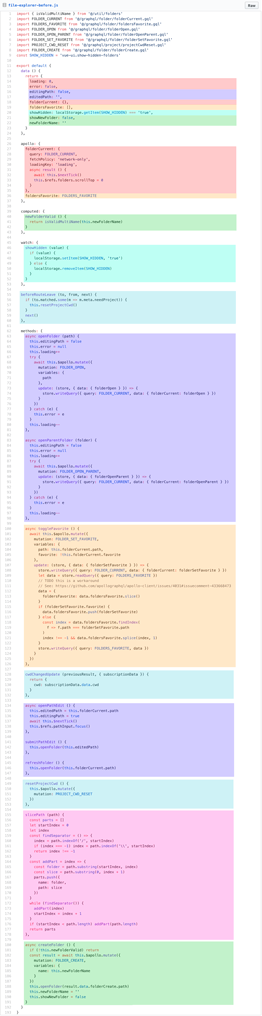
\includegraphics{./img/62783021-7ce24400-ba89-11e9-9dd3-36f4f6b1fae2.png} 
\end{center}
    

\columnratio{0.55}
\begin{paracol}{2} 
 
\switchcolumn[0]*%%%%%%%
Notice how code dealing with the same logical concern is forced to be
split under different options, located in different parts of the file.
In a component that is several hundred lines long, understanding and
navigating a single logical concern requires constantly scrolling up and
down the file, making it much more difficult than it should be. In
addition, if we ever intend to extract a logical concern into a reusable
utility, it takes quite a bit of work to find and extract the right
pieces of code from different parts of the file.
\switchcolumn
你可以看到,处理相同逻辑关注点的代码被强制拆分在了不同的选项中,位于文件的不同部分。在一个几百行的大组件中,要读懂代码中的一个逻辑关注点,需要在文件中反复上下滚动,这并不理想。另外,如果我们想要将一个逻辑关注点抽取重构到一个可复用的工具函数中,需要从文件的多个不同部分找到所需的正确片段。
\switchcolumn[0]*%%%%%%%
Here's the same component, before and after the
\href{https://gist.github.com/yyx990803/8854f8f6a97631576c14b63c8acd8f2e}{refactor
into Composition API}:
\switchcolumn
而如果\href{https://gist.github.com/yyx990803/8854f8f6a97631576c14b63c8acd8f2e}{用组合式
API 重构}这个组件,将会变成下面右边这样:
\end{paracol}

\begin{center} 
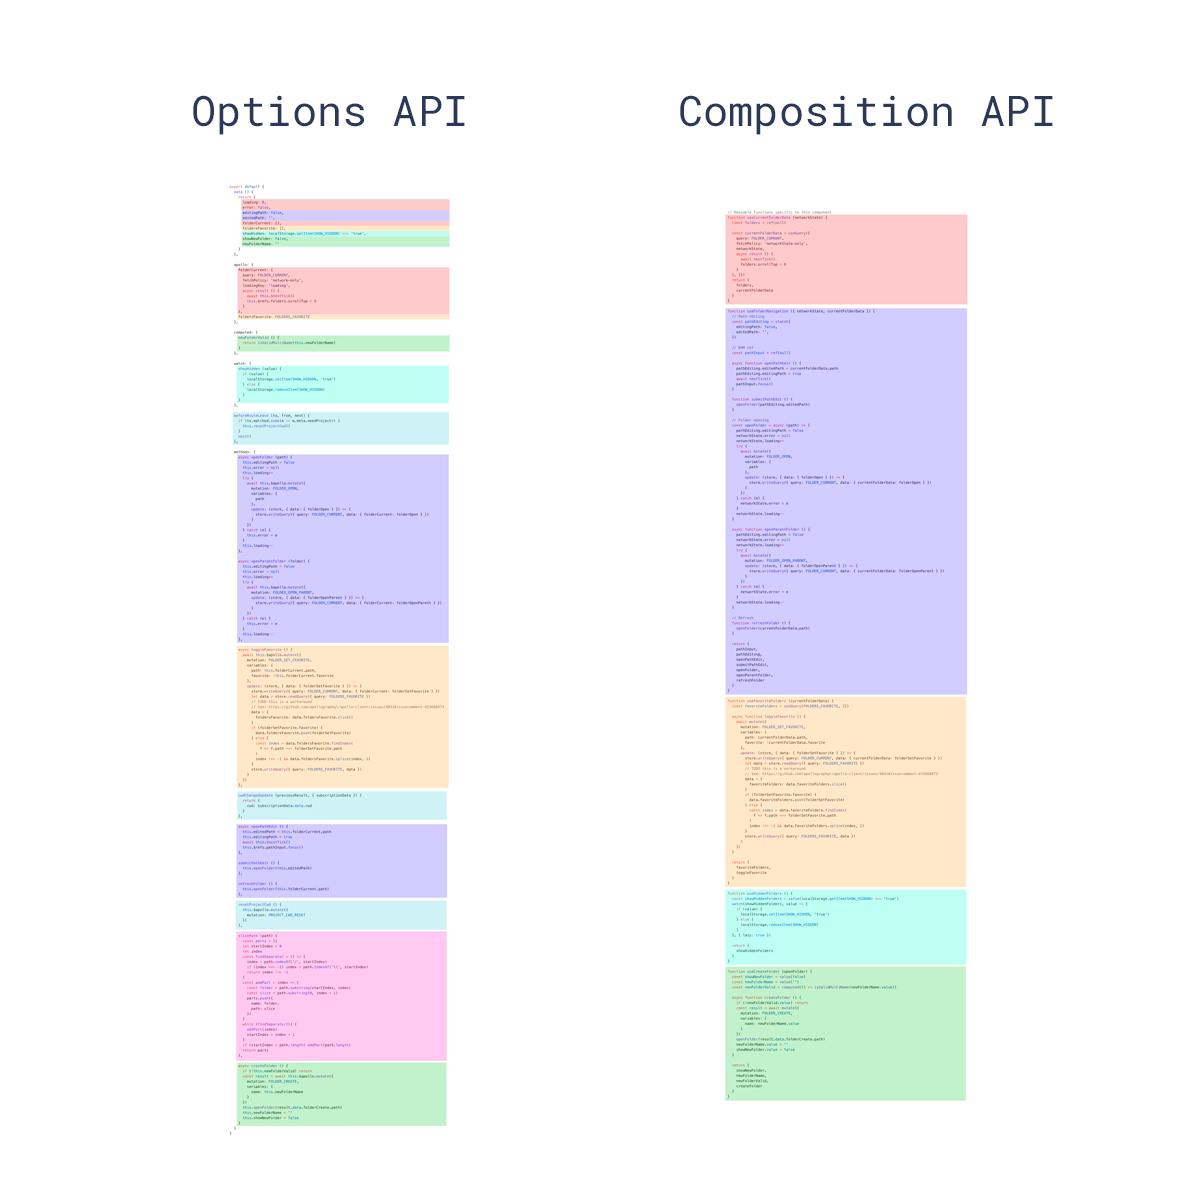
\includegraphics{./img/62783026-810e6180-ba89-11e9-8774-e7771c8095d6.png} 
\end{center}
     

\columnratio{0.55}
\begin{paracol}{2} 
 
\switchcolumn[0]*%%%%%%%
Notice how the code related to the same logical concern can now be
grouped together: we no longer need to jump between different options
blocks while working on a specific logical concern. Moreover, we can now
move a group of code into an external file with minimal effort, since we
no longer need to shuffle the code around in order to extract them. This
reduced friction for refactoring is key to the long-term maintainability
in large codebases.
\switchcolumn
现在与同一个逻辑关注点相关的代码被归为了一组:我们无需再为了一个逻辑关注点在不同的选项块间来回滚动切换。此外,我们现在可以很轻松地将这一组代码移动到一个外部文件中,不再需要为了抽象而重新组织代码,大大降低了重构成本,这在长期维护的大型项目中非常关键。 
\end{paracol}



\columnratio{0.55}
\begin{paracol}{2} 
 
\switchcolumn[0]*%%%%%%%
\subsubsection{Better Type Inference}
\switchcolumn
\subsubsection{更好的类型推导}
\switchcolumn[0]*%%%%%%%
In recent years, more and more frontend developers are adopting
\href{https://www.typescriptlang.org/}{TypeScript} as it helps us write
more robust code, make changes with more confidence, and provides a
great development experience with IDE support. However, the Options API,
originally conceived in 2013, was designed without type inference in
mind. We had to implement some
\href{https://github.com/vuejs/core/blob/44b95276f5c086e1d88fa3c686a5f39eb5bb7821/packages/runtime-core/src/componentPublicInstance.ts\#L132-L165}{absurdly
complex type gymnastics} to make type inference work with the Options
API. Even with all this effort, type inference for Options API can still
break down for mixins and dependency injection.
\switchcolumn
近几年来,越来越多的开发者开始使用
\href{https://www.typescriptlang.org/}{TypeScript}
书写更健壮可靠的代码,TypeScript 还提供了非常好的 IDE
开发支持。然而选项式 API 是在 2013
年被设计出来的,那时并没有把类型推导考虑进去,因此我们不得不做了一些\href{https://github.com/vuejs/core/blob/44b95276f5c086e1d88fa3c686a5f39eb5bb7821/packages/runtime-core/src/componentPublicInstance.ts\#L132-L165}{复杂到夸张的类型体操}才实现了对选项式
API 的类型推导。但尽管做了这么多的努力,选项式 API 的类型推导在处理
mixins 和依赖注入类型时依然不甚理想。
\switchcolumn[0]*%%%%%%%
This had led many developers who wanted to use Vue with TS to lean
towards Class API powered by \texttt{vue-class-component}. However, a
class-based API heavily relies on ES decorators, a language feature that
was only a stage 2 proposal when Vue 3 was being developed in 2019. We
felt it was too risky to base an official API on an unstable proposal.
Since then, the decorators proposal has gone through yet another
complete overhaul, and finally reached stage 3 in 2022. In addition,
class-based API suffers from logic reuse and organization limitations
similar to Options API.
\switchcolumn
因此,很多想要搭配 TS 使用 Vue 的开发者采用了由
\texttt{vue-class-component} 提供的 Class API。然而,基于 Class 的 API
非常依赖 ES 装饰器,在 2019 年我们开始开发 Vue 3 时,它仍是一个仅处于
stage 2 的语言功能。我们认为基于一个不稳定的语言提案去设计框架的核心 API
风险实在太大了,因此没有继续向 Class API
的方向发展。在那之后装饰器提案果然又发生了很大的变动,在 2022
年才终于到达 stage 3。另一个问题是,基于 Class 的 API 和选项式 API
在逻辑复用和代码组织方面存在相同的限制。
\switchcolumn[0]*%%%%%%%
In comparison, Composition API utilizes mostly plain variables and
functions, which are naturally type friendly. Code written in
Composition API can enjoy full type inference with little need for
manual type hints. Most of the time, Composition API code will look
largely identical in TypeScript and plain JavaScript. This also makes it
possible for plain JavaScript users to benefit from partial type
inference.
\switchcolumn
相比之下,组合式 API
主要利用基本的变量和函数,它们本身就是类型友好的。用组合式 API
重写的代码可以享受到完整的类型推导,不需要书写太多类型标注。大多数时候,用
TypeScript 书写的组合式 API 代码和用 JavaScript
写都差不太多!这也让许多纯 JavaScript 用户也能从 IDE
中享受到部分类型推导功能。
\switchcolumn[0]*%%%%%%%
\subsubsection{Smaller Production Bundle and Less Overhead}
\switchcolumn
\subsubsection{更小的生产包体积}
\switchcolumn[0]*%%%%%%%
Code written in Composition API and
\texttt{\textless{}script\ setup\textgreater{}} is also more efficient
and minification-friendly than Options API equivalent. This is because
the template in a \texttt{\textless{}script\ setup\textgreater{}}
component is compiled as a function inlined in the same scope of the
\texttt{\textless{}script\ setup\textgreater{}} code. Unlike property
access from \texttt{this}, the compiled template code can directly
access variables declared inside
\texttt{\textless{}script\ setup\textgreater{}}, without an instance
proxy in between. This also leads to better minification because all the
variable names can be safely shortened.
\switchcolumn
搭配 \texttt{\textless{}script\ setup\textgreater{}} 使用组合式 API
比等价情况下的选项式 API 更高效,对代码压缩也更友好。这是由于
\texttt{\textless{}script\ setup\textgreater{}}
形式书写的组件模板被编译为了一个内联函数,和
\texttt{\textless{}script\ setup\textgreater{}}
中的代码位于同一作用域。不像选项式 API 需要依赖 \texttt{this}
上下文对象访问属性,被编译的模板可以直接访问
\texttt{\textless{}script\ setup\textgreater{}}
中定义的变量,无需从实例中代理。这对代码压缩更友好,因为本地变量的名字可以被压缩,但对象的属性名则不能。
\switchcolumn[0]*%%%%%%%
\subsection{Relationship with Options API}
\switchcolumn
\subsection{与选项式 API 的关系}
\switchcolumn[0]*%%%%%%%
\subsubsection{Trade-offs}
\switchcolumn
\subsubsection{取舍}
\switchcolumn[0]*%%%%%%%
Some users moving from Options API found their Composition API code less
organized, and concluded that Composition API is "worse" in terms of
code organization. We recommend users with such opinions to look at that
problem from a different perspective.
\switchcolumn
一些从选项式 API 迁移来的用户发现,他们的组合式 API
代码缺乏组织性,并得出了组合式 API
在代码组织方面``更糟糕''的结论。我们建议持有这类观点的用户换个角度思考这个问题。    
\switchcolumn[0]*%%%%%%%
It is true that Composition API no longer provides the "guard rails"
that guide you to put your code into respective buckets. In return, you
get to author component code like how you would write normal JavaScript.
This means \textbf{you can and should apply any code organization best
practices to your Composition API code as you would when writing normal
JavaScript}. If you can write well-organized JavaScript, you should also
be able to write well-organized Composition API code.
\switchcolumn
组合式 API 不像选项式 API
那样会手把手教你该把代码放在哪里。但反过来,它却让你可以像编写普通的
JavaScript
那样来编写组件代码。这意味着\textbf{你能够,并且应该在写组合式 API
的代码时也运用上所有普通 JavaScript
代码组织的最佳实践}。如果你可以编写组织良好的
JavaScript,你也应该有能力编写组织良好的组合式 API 代码。
\switchcolumn[0]*%%%%%%%
Options API does allow you to "think less" when writing component code,
which is why many users love it. However, in reducing the mental
overhead, it also locks you into the prescribed code organization
pattern with no escape hatch, which can make it difficult to refactor or
improve code quality in larger scale projects. In this regard,
Composition API provides better long term scalability.
\switchcolumn
选项式 API
确实允许你在编写组件代码时``少思考'',这是许多用户喜欢它的原因。然而,在减少费神思考的同时,它也将你锁定在规定的代码组织模式中,没有摆脱的余地,这会导致在更大规模的项目中难以进行重构或提高代码质量。在这方面,组合式
API 提供了更好的长期可维护性。
\switchcolumn[0]*%%%%%%%
\subsubsection{Does Composition API cover all use cases?}
\switchcolumn
\subsubsection{组合式 API 是否覆盖了所有场景?}
\switchcolumn[0]*%%%%%%%
Yes in terms of stateful logic. When using Composition API, there are
only a few options that may still be needed: \texttt{props},
\texttt{emits}, \texttt{name}, and \texttt{inheritAttrs}.
\switchcolumn
组合式 API
能够覆盖所有状态逻辑方面的需求。除此之外,只需要用到一小部分选项:\texttt{props},\texttt{emits},\texttt{name}
和 \texttt{inheritAttrs}。
\switchcolumn[0]*%%%%%%%
\begin{vueQuote}{TIP}
Since 3.3 you can directly use \texttt{defineOptions} in
\texttt{\textless{}script\ setup\textgreater{}} to set the component
name or \texttt{inheritAttrs} property
\end{vueQuote} 
\switchcolumn
\begin{vueQuote}{TIP}
从 3.3 开始你可以直接通过
\texttt{\textless{}script\ setup\textgreater{}} 中的
\texttt{defineOptions} 来设置组件名或 \texttt{inheritAttrs} 属性。
\end{vueQuote} 
\switchcolumn[0]*%%%%%%%
If you intend to exclusively use Composition API (along with the options
listed above), you can shave a few kbs off your production bundle via a
\href{https://github.com/vuejs/core/tree/main/packages/vue\#bundler-build-feature-flags}{compile-time
flag} that drops Options API related code from Vue. Note this also
affects Vue components in your dependencies.
\switchcolumn
如果你在代码中只使用了组合式 API
(以及上述必需的选项),那么你可以通过配置\href{https://github.com/vuejs/core/tree/main/packages/vue\#bundler-build-feature-flags}{编译时标记}来去掉
Vue 运行时中针对选项式 API 支持的代码,从而减小生产包大概几 kb
左右的体积。注意这个配置也会影响你依赖中的 Vue 组件。
\end{paracol}



\columnratio{0.55}
\begin{paracol}{2} 
 
\switchcolumn[0]*%%%%%%%
\subsubsection{Can I use both APIs in the same component?}
\switchcolumn
\subsubsection{可以在同一个组件中使用两种 API 吗?}
\switchcolumn[0]*%%%%%%%
Yes. You can use Composition API via the
\href{https://vuejs.org/api/composition-api-setup.html}{\texttt{setup()}}
option in an Options API component.
\switchcolumn
可以。你可以在一个选项式 API 的组件中通过
\href{https://cn.vuejs.org/api/composition-api-setup.html}{\texttt{setup()}}
选项来使用组合式 API。
\switchcolumn[0]*%%%%%%%
However, we only recommend doing so if you have an existing Options API
codebase that needs to integrate with new features / external libraries
written with Composition API.
\switchcolumn
然而,我们只推荐你在一个已经基于选项式 API
开发了很久、但又需要和基于组合式 API
的新代码或是第三方库整合的项目中这样做。
\switchcolumn[0]*%%%%%%%
\subsubsection{Will Options API be deprecated?}
\switchcolumn
\subsubsection{选项式 API 会被废弃吗?}
\switchcolumn[0]*%%%%%%%
No, we do not have any plan to do so. Options API is an integral part of
Vue and the reason many developers love it. We also realize that many of
the benefits of Composition API only manifest in larger-scale projects,
and Options API remains a solid choice for many low-to-medium-complexity
scenarios.
\switchcolumn
不会,我们没有任何计划这样做。选项式 API 也是 Vue
不可分割的一部分,也有很多开发者喜欢它。我们也意识到组合式 API
更适用于大型的项目,而对于中小型项目来说选项式 API
仍然是一个不错的选择。
\switchcolumn[0]*%%%%%%%
\subsection{Relationship with Class API}
\switchcolumn
\subsection{与 Class API 的关系}
\switchcolumn[0]*%%%%%%%
We no longer recommend using Class API with Vue 3, given that
Composition API provides great TypeScript integration with additional
logic reuse and code organization benefits.
\switchcolumn
我们不再推荐在 Vue 3 中使用 Class API,因为组合式 API 提供了很好的
TypeScript 集成,并具有额外的逻辑重用和代码组织优势。
\switchcolumn[0]*%%%%%%%
\subsection{Comparison with React Hooks}
\switchcolumn
\subsection{和 React Hooks 的对比}
\switchcolumn[0]*%%%%%%%
Composition API provides the same level of logic composition
capabilities as React Hooks, but with some important differences.
\switchcolumn
组合式 API 提供了和 React Hooks
相同级别的逻辑组织能力,但它们之间有着一些重要的区别。
\switchcolumn[0]*%%%%%%%
React Hooks are invoked repeatedly every time a component updates. This
creates a number of caveats that can confuse even seasoned React
developers. It also leads to performance optimization issues that can
severely affect development experience. Here are some examples:
\switchcolumn
React Hooks 在组件每次更新时都会重新调用。这就产生了一些即使是经验丰富的
React
开发者也会感到困惑的问题。这也带来了一些性能问题,并且相当影响开发体验。例如:
\switchcolumn[0]*%%%%%%%
\begin{itemize}
\item
  Hooks are call-order sensitive and cannot be conditional.
\item
  Variables declared in a React component can be captured by a hook
  closure and become "stale" if the developer fails to pass in the
  correct dependencies array. This leads to React developers relying on
  ESLint rules to ensure correct dependencies are passed. However, the
  rule is often not smart enough and over-compensates for correctness,
  which leads to unnecessary invalidation and headaches when edge cases
  are encountered.
\item
  Expensive computations require the use of \texttt{useMemo}, which
  again requires manually passing in the correct dependencies array.
\item
  Event handlers passed to child components cause unnecessary child
  updates by default, and require explicit \texttt{useCallback} as an
  optimization. This is almost always needed, and again requires a
  correct dependencies array. Neglecting this leads to over-rendering
  apps by default and can cause performance issues without realizing it.
\item
  The stale closure problem, combined with Concurrent features, makes it
  difficult to reason about when a piece of hooks code is run, and makes
  working with mutable state that should persist across renders (via
  \texttt{useRef}) cumbersome.
\end{itemize}
\switchcolumn
\begin{itemize}
\item
  Hooks 有严格的调用顺序,并不可以写在条件分支中。
\item
  React
  组件中定义的变量会被一个钩子函数闭包捕获,若开发者传递了错误的依赖数组,它会变得``过期''。这导致了
  React 开发者非常依赖 ESLint
  规则以确保传递了正确的依赖,然而,这些规则往往不够智能,保持正确的代价过高,在一些边缘情况时会遇到令人头疼的、不必要的报错信息。
\item
  昂贵的计算需要使用 \texttt{useMemo},这也需要传入正确的依赖数组。
\item
  在默认情况下,传递给子组件的事件处理函数会导致子组件进行不必要的更新。子组件默认更新,并需要显式的调用
  \texttt{useCallback}
  作优化。这个优化同样需要正确的依赖数组,并且几乎在任何时候都需要。忽视这一点会导致默认情况下对应用进行过度渲染,并可能在不知不觉中导致性能问题。
\item
  要解决变量闭包导致的问题,再结合并发功能,使得很难推理出一段钩子代码是什么时候运行的,并且很不好处理需要在多次渲染间保持引用
  (通过 \texttt{useRef}) 的可变状态。
\end{itemize}
\switchcolumn[0]*%%%%%%%
In comparison, Vue Composition API:
\switchcolumn
相比起来,Vue 的组合式 API:
\switchcolumn[0]*%%%%%%%
\begin{itemize}
\item
  Invokes \texttt{setup()} or
  \texttt{\textless{}script\ setup\textgreater{}} code only once. This
  makes the code align better with the intuitions of idiomatic
  JavaScript usage as there are no stale closures to worry about.
  Composition API calls are also not sensitive to call order and can be
  conditional.
\item
  Vue's runtime reactivity system automatically collects reactive
  dependencies used in computed properties and watchers, so there's no
  need to manually declare dependencies.
\item
  No need to manually cache callback functions to avoid unnecessary
  child updates. In general, Vue's fine-grained reactivity system
  ensures child components only update when they need to. Manual
  child-update optimizations are rarely a concern for Vue developers.
\end{itemize}
\switchcolumn
\begin{itemize}
\item
  仅调用 \texttt{setup()} 或
  \texttt{\textless{}script\ setup\textgreater{}}
  的代码一次。这使得代码更符合日常 JavaScript
  的直觉,不需要担心闭包变量的问题。组合式 API
  也并不限制调用顺序,还可以有条件地进行调用。
\item
  Vue
  的响应性系统运行时会自动收集计算属性和侦听器的依赖,因此无需手动声明依赖。
\item
  无需手动缓存回调函数来避免不必要的组件更新。Vue
  细粒度的响应性系统能够确保在绝大部分情况下组件仅执行必要的更新。对 Vue
  开发者来说几乎不怎么需要对子组件更新进行手动优化。
\end{itemize}
\switchcolumn[0]*%%%%%%%
We acknowledge the creativity of React Hooks, and it is a major source
of inspiration for Composition API. However, the issues mentioned above
do exist in its design and we noticed Vue's reactivity model happens to
provide a way around them.
\switchcolumn
我们承认 React Hooks 的创造性,它是组合式 API
的一个主要灵感来源。然而,它的设计也确实存在上面提到的问题,而 Vue
的响应性模型恰好提供了一种解决这些问题的方法。
\end{paracol}


\columnratio{0.55}
\begin{paracol}{2} 

\end{paracol}



\columnratio{0.55}
\begin{paracol}{2} 

\end{paracol}



\columnratio{0.55}
\begin{paracol}{2} 

\end{paracol}


\columnratio{0.55}
\begin{paracol}{2} 

\end{paracol}



\columnratio{0.55}
\begin{paracol}{2} 

\end{paracol}



\columnratio{0.55}
\begin{paracol}{2} 

\end{paracol}



\columnratio{0.55}
\begin{paracol}{2} 

\end{paracol}



\columnratio{0.55}
\begin{paracol}{2} 

\end{paracol}



\columnratio{0.55}
\begin{paracol}{2} 

\end{paracol}


\columnratio{0.55}
\begin{paracol}{2} 

\end{paracol}



\columnratio{0.55}
\begin{paracol}{2} 

\end{paracol}



\columnratio{0.55}
\begin{paracol}{2} 

\end{paracol}


\columnratio{0.55}
\begin{paracol}{2} 

\end{paracol}



\columnratio{0.55}
\begin{paracol}{2} 

\end{paracol}